\chapter{Simulation Study} \label{chapter3:Simulation-Study}

In this chapter we will present some results that compare the method presented in Chapter~\ref{chapter2:Procedure}, which we will refer to as the ``spline method,'' to some existing techniques for estimating covariance functions. In Section~\ref{sec:comparing_exact_and_estimated_log_likelihoods}, we examine the accuracy of the likelihood estimate from Algorithm~\ref{alg:lik}. In Sections~\ref{sec:prediction_performance} and \ref{sec:covariance_function_estimation_performance}, we compare the spline method to existing methods with regard to prediction performance and how closely they estimate the true covariance function, respectively.

\section{Comparing Exact and Estimated Log Likelihoods} % (fold)
\label{sec:comparing_exact_and_estimated_log_likelihoods}

Assume we observe $\bm{y} = (y_1, \dots, y_{400})^T$ from a Gaussian process where the covariance function is Mat\'{e}rn (see \eqref{eq:matern}) with known parameters $\nu$, $\rho$, and $\sigma$. The observations come from locations $\bm{s}_1, \dots, \bm{s}_{400}$ spread randomly over the unit square in $\mathbb{R}^2$. Because we know $C(h)$, we can calculate the covariance matrix exactly:
\[
	\bm{\Sigma}_{ij} = C(||\bm{s}_i - \bm{s}_j||).
\]
From this we can find the exact likelihood.

The spectral density corresponding to the Mat\'{e}rn covariance function \eqref{eq:matern}, is
\[
	f(\omega) = \frac{\sigma g(\nu, \rho)}{\big( \frac{4\nu}{\rho^2} + \omega^2 \big)^{\nu+d/2}},
\]
where $d = 2$ is the dimension of the spatial domain and
\[
	g(\nu, \rho) = \frac{\Gamma\left(\nu + \frac{d}{2}\right)(4\nu)^\nu}{\pi^{d/2} \rho^{2\nu} \Gamma(\nu)}.
\]
Because we can calculate the spectral density directly in this scenario, we can avoid fitting the splines and estimating $\bm{\beta}$. By bypassing this step, we test just the procedures for sampling from $f(\omega)$ and estimating the log likelihood.

To perform the test, we chose two values for $\nu$ and six values for $\rho$. The $\sigma^2$ parameter just controls the marginal variance $\textrm{Var}(\bm{Y}(\bm{s}))$, and so it can be factored out of the covariance matrix $\bm{\Sigma}$. For each combination of parameter settings, we generated 100 Gaussian process realizations and compared the true and estimated log likelihoods. The results are summarized in Figure~\ref{fig:liks_by_rho}. Note that the estimated likelihoods are close to their true values in all cases, and the choice of $\rho$ does not appear to significantly affect the accuracy.

\begin{figure}[!htb]
	\centering
	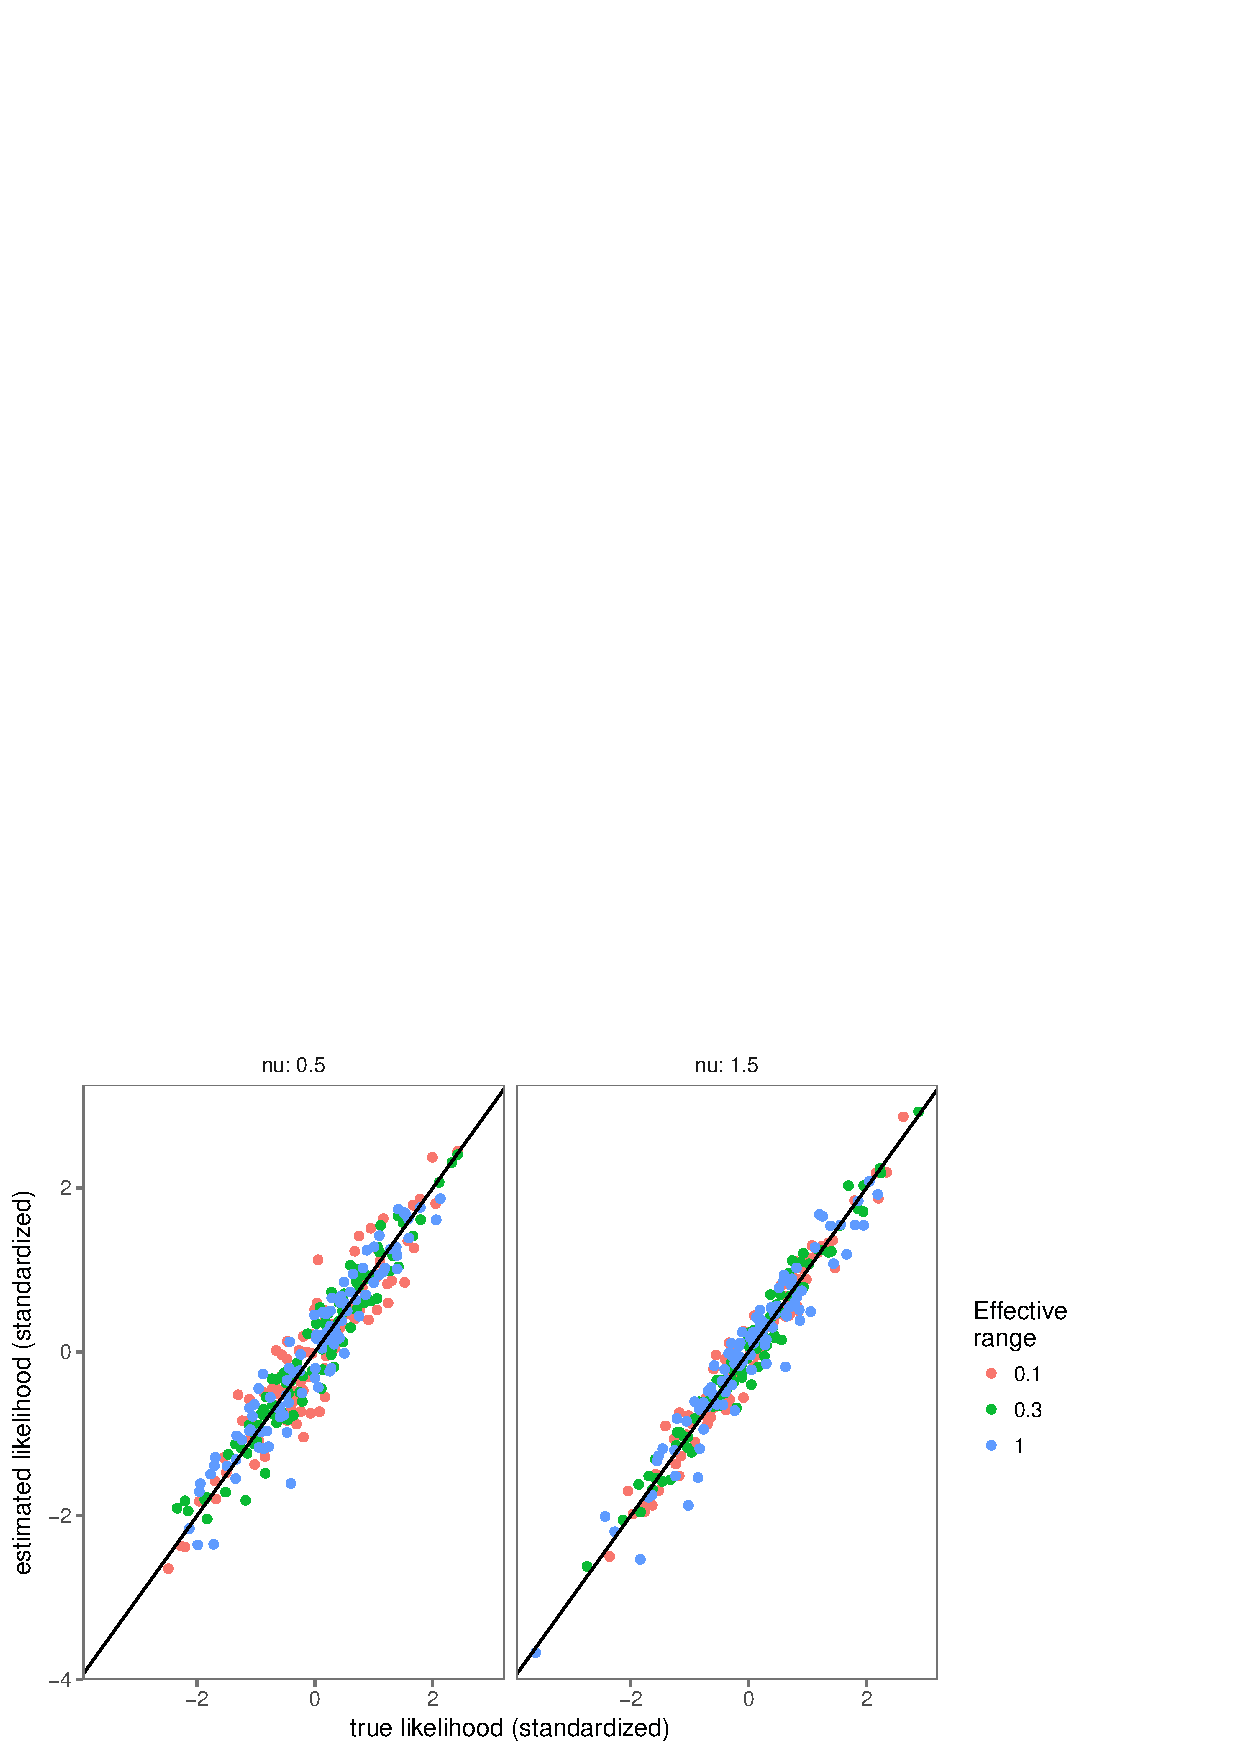
\includegraphics[width=0.95\textwidth]{lik_true_vs_est.pdf}
	\caption{\small Comparing true and estimated log likelihoods for varying values of $\rho$ (given above each plot). Values in each plot were centered and scaled for easier comparison. The likelihoods for the two values of $\nu$, $0.5$ and $1.5$, yield a similar pattern.}
	\label{fig:liks_by_rho}
\end{figure}

% \begin{figure}[htbp]
% 	\centering
% 	\includegraphics[width=0.95\textwidth]{rel_ll_err_1.pdf}
% 	\caption{Relative error of the estimated log likelihood. Samples came directly from the true spectral density $f(\omega)$. Each facet of the plot corresponds to different effective ranges (0.1, 0.3, 1), and contains a boxplot for each of $\nu = 0.5$ and $\nu = 1.5$. Every boxplot is made from 100 different datasets.}
% 	\label{fig:rel-ll-err-1}
% \end{figure}

We ran a second version of this test that incorporated the $\bm{\beta}$ estimation. Still assuming the true $f(\omega)$ is known, we took 50 equally spaced points along $\log f(\log \omega)$ and fit natural splines to those points. This gave me some $\bm{\beta}_{\textrm{opt}}$, the values for $\bm{\beta}$ that most closely approximate $\log f(\log \omega)$. Then using $\bm{\beta}_{\textrm{opt}}$ we estimated the likelihood and again compared it to the true likelihood. Results are shown in Figure~\ref{fig:estliks_spline_rho}. The estimated likelihoods are still comparable to their true values, despite the fact that we are sampling from a spline approximation to $f(\omega)$ rather than $f(\omega)$ itself.

\begin{figure}[!htb]
	\centering
	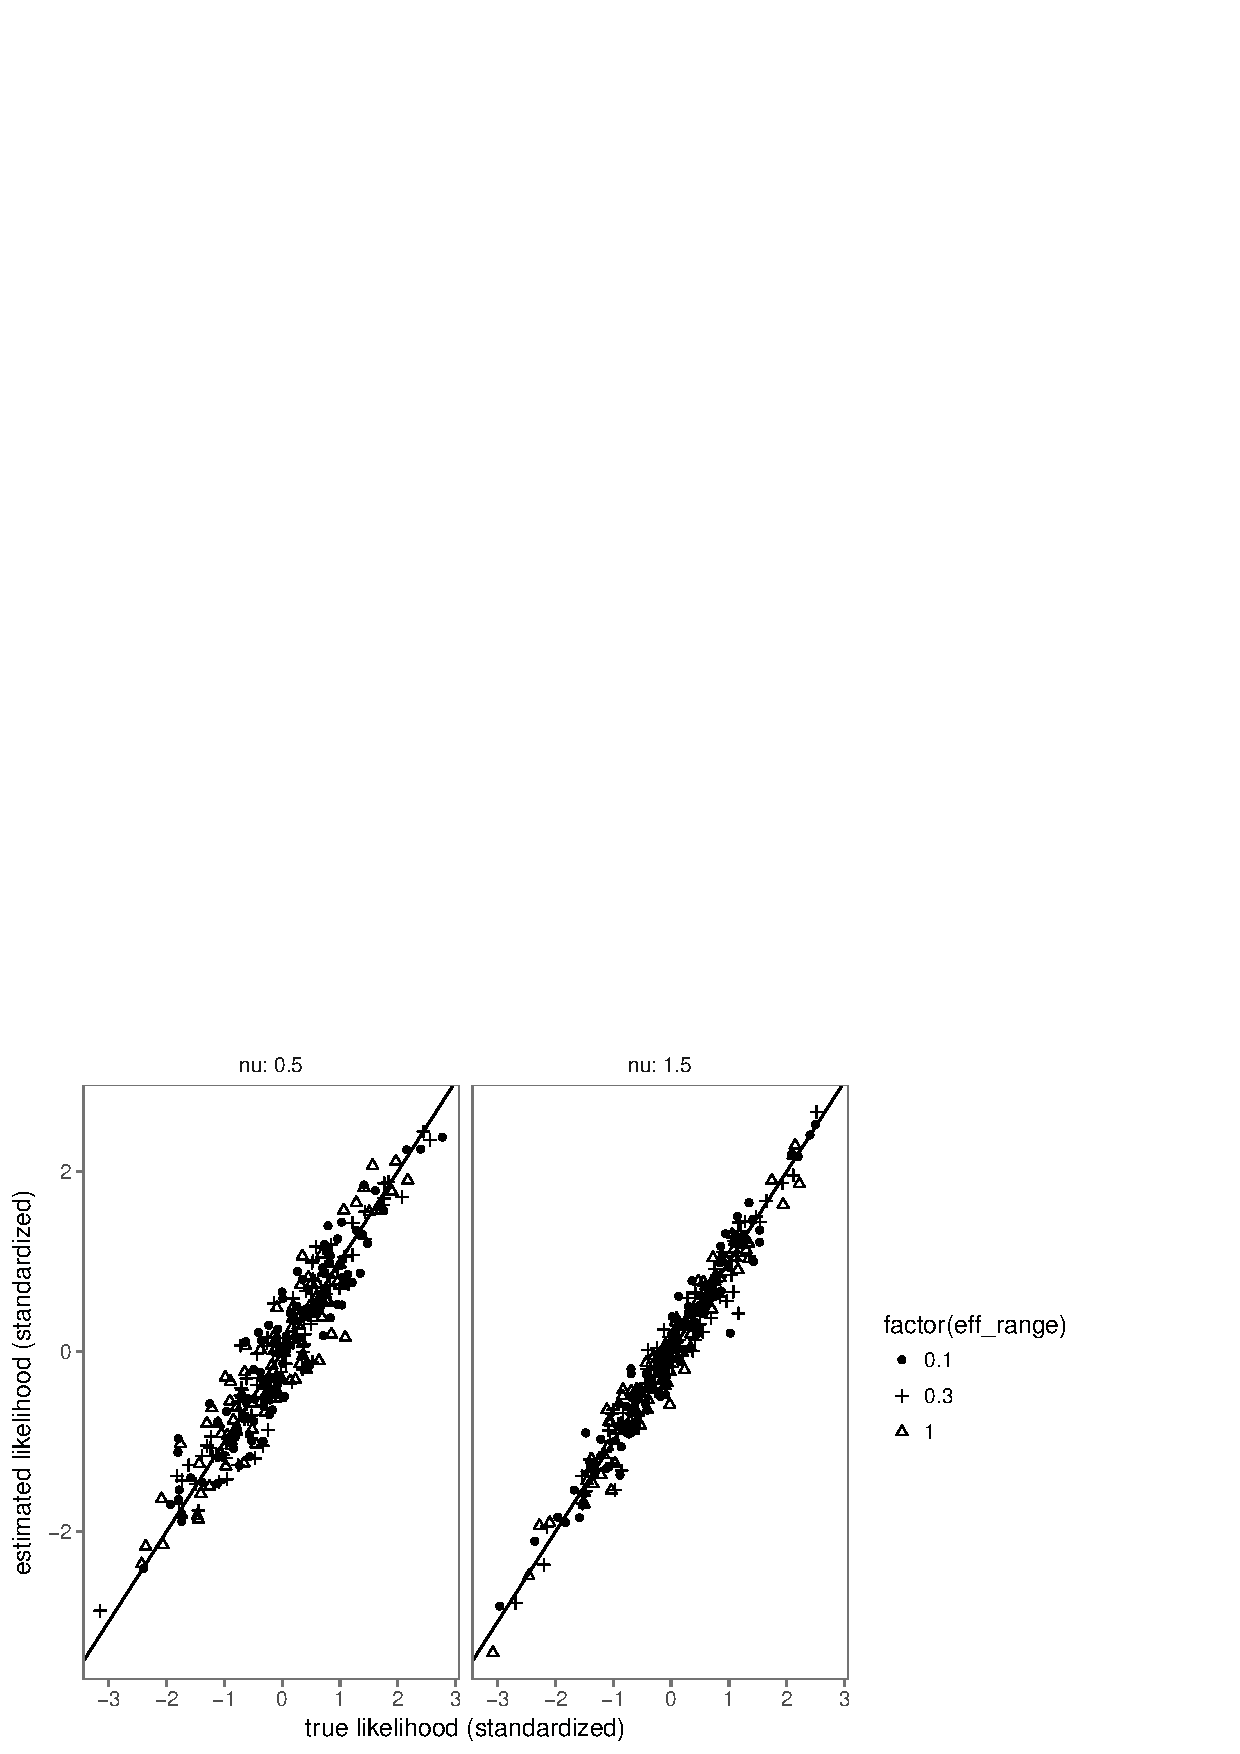
\includegraphics[width=0.95\textwidth]{lik_true_vs_est2.pdf}
	\caption{\small Comparing true and estimated log likelihoods for varying values of $\rho$ (given above each plot). Unlike the results in Figure~\ref{fig:liks_by_rho}, these estimates were generated not by sampling from $f(\omega)$ directly, but by sampling from a density approximating $f(\omega)$ fit using splines.}
	\label{fig:estliks_spline_rho}
\end{figure}

% \begin{figure}[htbp]
% 	\centering
% 	\includegraphics[width=0.95\textwidth]{rel_ll_err_2.pdf}
% 	\caption{Relative error of the estimated log likelihood. Unlike the results in Figure~\ref{fig:liks_by_rho}, these estimates were generated not by sampling from $f(\omega)$ directly, but by sampling from a density approximating $f(\omega)$ fit using splines. Each facet of the plot corresponds to different effective ranges (0.1, 0.3, 1), and contains a boxplot for each of $\nu = 0.5$ and $\nu = 1.5$. Every boxplot is made from 100 different datasets.}
% 	\label{fig:rel-ll-err-2}
% \end{figure}

\begin{figure}[htbp]
	\centering
	\includegraphics[width=0.95\textwidth]{est_vs_true_8_0-5_2.png}
	\caption{Posterior distributions of $\rho|\bm{y}$ for the true likelihood function and our estimated likelihood. This plot shows $\alpha$, which occurs in another parameterization of the Mat\'ern covariance function and is simply $1/\rho$. The observations were simulated with a value of $\alpha = 8$, but the maximum likelihood estimate given the data was $\hat{\alpha}_{MLE} = 10.32$.}
	\label{fig:compare-one}
\end{figure}

As an additional test that we are correctly estimating the true likelihood, we simulated another set of 400 observations $\bm{y} = (y_1, \dots, y_{400})^T$ from a Gaussian process with Mat\'ern covariance function. We treat $\rho$ and $\nu$ as fixed and known, and used MCMC to find the posterior distribution of $\rho|\bm{y}$ using the true likelihood function, and again using the estimated likelihood from Algorithm~\ref{alg:lik}. One result from this test is shown in Figure~\ref{fig:compare-one}. We see that the two posterior distributions are very similar, futher indicating that our likelihood estimate is reasonable for use in our more complicated semiparametric MCMC (Algorithm~\ref{alg:mcmc}).

\section{Prediction Performance} % (fold)
\label{sec:prediction_performance}

Next, we put the entire procedure from Algorithm~\ref{alg:mcmc} into motion. First, $n = 400$ observations $\bm{y} = (y_1, \dots, y_{400})^T$ are drawn from a Gaussian process with a Mat\`{e}rn covariance function with $\nu = 1.5$, $\rho = 0.1548$, and $\sigma = 1$. This particular value of $\rho$ was chosen to obtain an effective range of 0.3. The observation locations are randomly spread across the unit square in $\mathbb{R}^2$ (see Figure~\ref{fig:locations}). An arbitrary initial $\bm{\beta}_0$ is chosen, and Algorithm~\ref{alg:mcmc} is run for $10000$ iterations. At each iteration $i$, one likelihood calculation is made, using $M = 50000$ samples from the spectral density $f_{\bm{\beta}(i)}(\omega)$. After the chain is finished, the accepted $\bm{\beta}$ values are samples from the posterior distribution of $\bm{\beta} \;|\; \bm{y}$. After throwing away the first $2000$ values in the chain as burnin, the posterior mean $\widehat{\bm{\beta}}$ is chosen to be the best estimate of the true $\bm{\beta}$.

We chose a normal random walk proposal distribution for both the $\bm{\beta}$ and $\tau^2$ updates. Because it is symmetric, we were able to omit the proposal density from the calculation of the ratio $a$ in Algorithm~\ref{alg:mcmc}. We also used adaptive tuning to adjust the hyperparameters so that the acceptance rates stayed within an acceptable range.

Because we know the true $f(\omega)$, we can compare the spectral density approximated with $\widehat{\bm{\beta}}$ with the actual one. See Figure~\ref{fig:result} for that comparison. Figure~\ref{fig:result-covar} shows that the estimated covariance function agrees with the actual covariance function.


\begin{figure}[!htb]
	\centering
	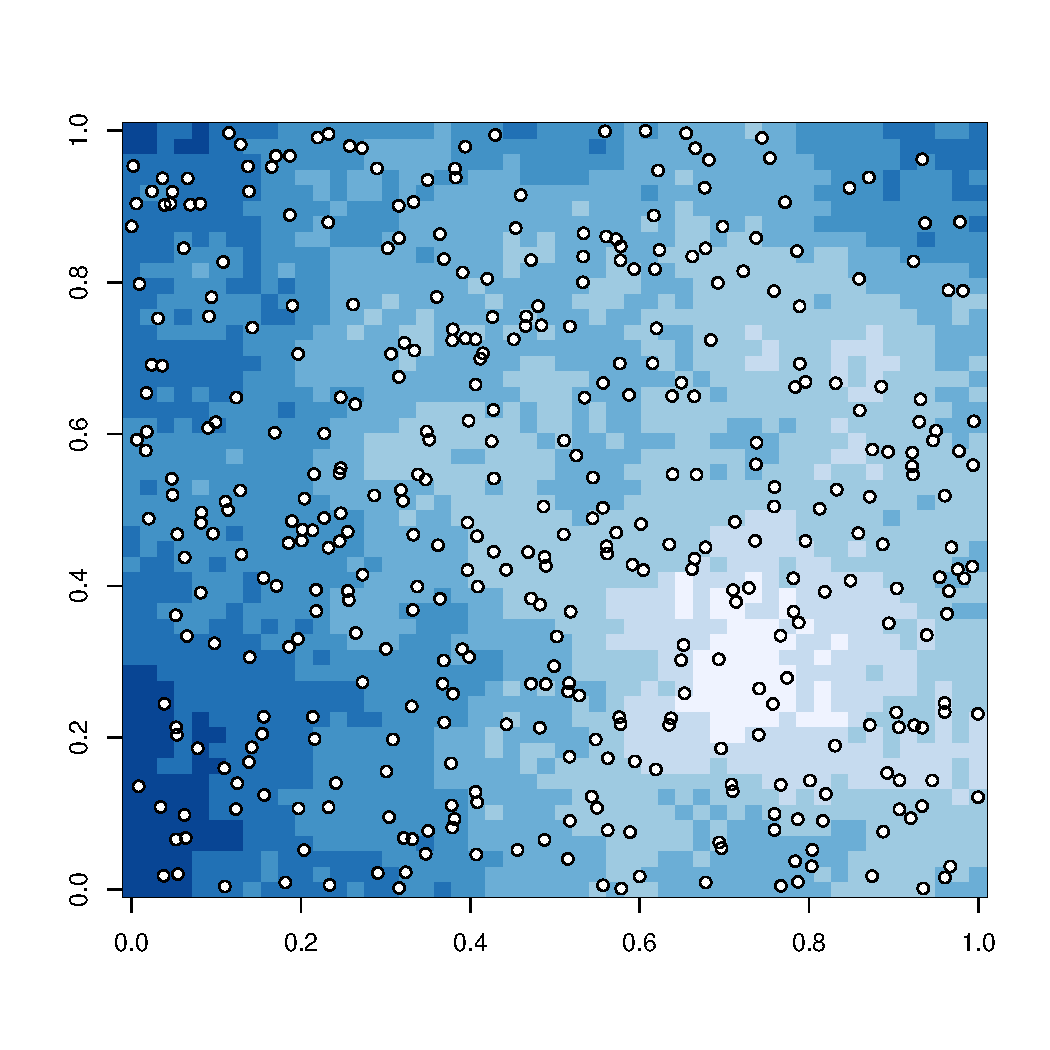
\includegraphics[width=0.95\textwidth]{locations.pdf}
	\caption{\small The locations $\bm{s}_1, \dots, \bm{s}_{400} \in \mathbb{R}^2$ of the observations from a Gaussian process with $\nu = 1.5$, $\rho = 0.1548$, and $\sigma = 1$. The locations are random, but generated in such a way that ensures the minimum distance between any two points is greater than $0.005$.}
	\label{fig:locations}
\end{figure}

\begin{figure}[!htb]
	\centering
	\includegraphics[width=0.95\textwidth]{logdensity2.pdf}
	\caption{\small The actual $f(\log \omega)$ (grey dots) versus the estimated $\hat{f}(\omega)$ (blue). The shaded area represents the range of the middle 95\% of $\hat{f}(\omega)$ for all draws from $\bm{\beta} \;|\; \bm{y}$. The vertical gray dotted lines indicate where the knots were placed.}
	\label{fig:result}
\end{figure}

\begin{figure}[!htb]
	\centering
	\includegraphics[width=0.95\textwidth]{covar.pdf}
	\caption{\small The actual $C(h)$ (black) versus the estimated $\widehat{C}(h)$ (blue). The shaded area represents the range of the middle 95\% of $\widehat{C}(h)$ for all draws from $\bm{\beta} \;|\; \bm{y}$.}
	\label{fig:result-covar}
\end{figure}

The overall simulation study was set up as follows: first we simulate 100 mean-zero Gaussian processes with Matern covariance functions ($\nu = 1.5, \rho = 0.1548, \sigma = 1$) and 100 mean-zero Gaussian processes with damped cosine covariance functions ($\lambda = 1, \tau = 1$) with 400 observations randomly placed over the unit square, as above. In addition, for every dataset, observations were generated over a $50\times50$ uniform grid. These were held out for prediction.

We compare three techniques. The first is the ``spline method'' from Chapter~\ref{chapter2:Procedure}. For the second, we fit a univariate Gaussian spatial regression model using the \texttt{spBayes} R package~\cite{spBayes1}~\cite{spBayes2}. This package's \texttt{spLM} function fits the model
\[
	y(\bm{s}) = \bm{x}(\bm{s})'\bm{\beta} + w(\bm{s}) + \varepsilon(\bm{s})
\]
using a Metropolis algorithm. See the package vignette for implementation details. In our case, we have no predictors $\bm{x}$, just the locations $\bm{s}$ themselves, so the model reduces to $y(\bm{s}) = w(\bm{s}) + \varepsilon(\bm{s})$, where $w$ is the spatial process and $\varepsilon$ is an independent white-noise process. We can specify that $w$ should employ a Mat\'{e}rn covariance function, and \texttt{spLM} can estimate the parameter values from \eqref{eq:matern}. In effect, this gives us the Mat\'{e}rn model that best fits the data.

The third technique is the one introduced by Hall et al.~\cite{Hall1994}. We find a kernel estimate of the covariogram using the kernel
\[
	K(x) = 0.9375(1 - x^2)^2
\]
as the authors do in their original paper. We then numerically calculate the Fourier transform of this covariagram estimate, set all values beyond the first nonnegative one to zero to ensure positive definiteness, and Fourier transform back to the spatial domain.

For each of these techniques, we estimate the covariance function using the 400 observations, generate predictions for the 2500 held out locations, and calculate the mean squared prediction error. We do this for every simulated dataset. Figure~\ref{fig:true-vs-est-all} shows the resulting covariance function estimates for every dataset, along with the true covariance functions. The Hall method underestimates the covariance at short distances in both the Mat\'{e}rn and damped cosine cases. Notice that the spline method is the only one to capture the hole effect in the damped cosine case, although it does tend to overestimate the magnitude of the effect.

\begin{figure}[htbp]
	\centering
	\includegraphics[width=0.95\textwidth]{true_vs_est_all.pdf}
	\caption{True covariance functions for the Mat\`{e}rn and damped cosine cases, along with all of the estimates. The spline method estimates are in blue, the Hall method is in green, and the best-fitting Mat\`{e}rn is in red.}
	\label{fig:true-vs-est-all}
\end{figure}

Finally, we examine the integrated mean-square prediction error (IMSPE). For each dataset, we calculate the \emph{optimal} IMSPE by generating predictions at each of the 2500 prediction locations according to the true covariance function, and then comparing them to the corresponding observations. The boxplots in Figure~\ref{fig:pred-log} show the IMSPE relative to this optimal value for every dataset. The IMSPE is shown on the log scale to make the boxplots a bit more readable relative to one another.

Notice that both the spline method and the best-fitting Mat\'{e}rn model outperform the Hall method with regard to prediction, and are fairly close to each other. As expected, the best-fitting Mat\'{e}rn performs the best when the true process was also Mat\'{e}rn. Interestingly, it performs a bit better than the spline method when the true process was not Mat\'{e}rn as well. This further validates the argument in~\cite{Stein1999} that the Mat\'{e}rn model is an excellent choice in most practical situations when prediction accuracy is the goal. It does not pick up the hole effect present at moderate distances in the damped cosine model (see Figure~\ref{fig:true-vs-est-all}), but interpolation is largely governed by the behavior at small distances, i.e. the smoothness of the process. The Mat\'{e}rn covariance function~\ref{eq:matern} has a parameter $\nu$ that controls this smoothness. Because we're estimating $\nu$ directly, we are able to precisely adjust it and get very good prediction performance.

There were a few Mat\'{e}rn datasets for which the spline method performed very poorly, as the long right tail of the boxplot indicates. This occurred when the Metropolis algorithm described in Algorithm~\ref{alg:mcmc} either mixed very poorly or started with poor initial $\bm{\beta}$ values. These issues could be corrected on any single dataset by manual intervention (e.g. by tuning the algorithm, running more iterations, etc.), but because the method was applied to all 100 datasets in bulk, we did not tune them individually. Note that these issues arose in only a few datasets, and the median relative IMSPE is still competitive with the best-fitting Mat\'{e}rn results.

\begin{figure}[htbp]
	\centering
	\includegraphics[width=0.95\textwidth]{pred_log.pdf}
	\caption{Mean squared prediction error relative to the optimal. The x axis is on the log scale, so the optimal MSPE would fall at zero.}
	\label{fig:pred-log}
\end{figure}

\section{Covariance Function Estimation Performance} % (fold)
\label{sec:covariance_function_estimation_performance}

We continue to evaluate these techniques by introducing another measure of performance. Broadly, we would like to know how closely the estimated covariance function aligns with the true covariance function. Let $C(h)$ be the true covariance and $\widehat{C}_m(h)$ be the estimate from method $m$. Define the function
\[
	g_m(h) = \big(C(h) - \widehat{C}_m(h) \big)^2.
\]
Then the integrated mean squared error with respect to method $m$ is
\[
	IMSE_m = \int_0^\infty g_m(h) \; dh.
\]
To approximate this integral, we evaluate $g_m(h)$ on a uniform grid $\{h_0, \dots, h_N\}$, $0 \leq h_i \leq 5$, and use the trapezoidal rule:
\[
	\widehat{IMSE}_m = \sum_{i=1}^N \frac{g_m(h_{i-1}) + g_m(h_i)}{2} (h_i - h_{i-1}).
\]
In Figure~\ref{fig:sqdiff}, the functions $g_m(h)$ are shown for all methods and both covariance function types.

\begin{figure}[htbp]
	\centering
	\includegraphics[width=0.95\textwidth]{sqdiff.pdf}
	\caption{Squared discrepancy functions $g_m(h)$ for every method, both Mat\'{e}rn and damped cosine covariance models. The result from each simulated dataset is shown in gray, and the thicker black lines are the means of each facet of the plot.}
	\label{fig:sqdiff}
\end{figure}

There are a number of interesting features of this figure. First of all, the squared difference functions of the best-fit Mat\'{e}rn model and the spline method are, for the most part, quite small in magnitude. This further confirms what we observed in Figure~\ref{fig:true-vs-est-all} that these two methods fit the true Mat\'{e}rn covariance function very well. The Hall method does not perform as well for small $h$, although it does recover and match the true function once $h$ is greater than 2. The best-fit Mat\'{e}rn tends to be slightly inaccurate for very small $h$, but its errors are smaller and it recovers even more quickly than the Hall method. On the other hand, the spline method appears to be at its most inaccurate not at $h = 0$, but around $0.25 < h < 1$.

Not surprisingly, the best-fit Mat\'{e}rn does not match the true covariance as well when the truth is not actually a Mat\'{e}rn covariance function. The spline method is closer to the truth, but it does tend to consistently overestimate the magnitude of the hole effect at $1 < h < 2$. The Hall method is the least accurate of the three on these data.

Figure~\ref{fig:boxplot-integrals} shows the IMSE (the integrals of the curves in Figure~\ref{fig:true-vs-est-all}) for all datasets. Again, the best-fit Mat\'{e}rn and the spline method performed comparably on the Mat\'{e}rn datasets, with the Hall method doing worse. For the damped cosine datasets, the spline method performed better on average than the best-fit Mat\'{e}rn.

\begin{figure}[htbp]
	\centering
	\includegraphics[width=0.95\textwidth]{boxplot_integrals2.pdf}
	\caption{Boxplots of IMSE by method.}
	\label{fig:boxplot-integrals}
\end{figure}

% section covariance_function_estimation_performance (end)